\chapter{Hydras and Hydra Games}
\label{sec:orgheadline91}

This chapter is dedicated to the representation of hydras and rules of the hydra game in \coq's specification language:\gallina. 

Technically, a \emph{hydra} is just a finite ordered tree, each node of which 
has any number of sons. Note that, contrary to the computer science tradition, we will show the hydras 
with the heads up and the foot (i.e., the root of the tree) down.
Fig.~\ref{fig:Hy} represents such  a hydra, which will be referred to as \texttt{Hy} in our examples (please look at the 
module~\href{../src/html/hydras.Hydra.Hydra_Examples.html}{Hydra.Hydra\_Examples}). 

\begin{figure}[h]
\centering
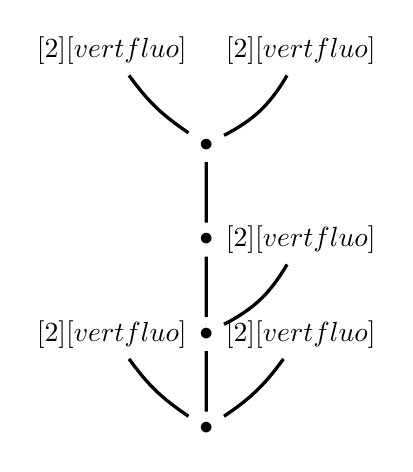
\begin{tikzpicture}[very thick, scale=0.6]

\node (foot) at (2,0) {$\bullet$};
\node (N1) at (2,2) {$\bullet$};
\node (N2) at (2,4) {$\bullet$};
\node (N3) at (2,6) {$\bullet$};
\node (H0) at (0,2) {$\Smiley[2][vertfluo]$};
\node (H1) at (0,8) {$\Smiley[2][vertfluo]$};
\node (H2) at (4,8) {$\Smiley[2][vertfluo]$};
\node (H4) at (4,2) {$\Smiley[2][vertfluo]$};
\node (H5) at (4,4) {$\Smiley[2][vertfluo]$};
\draw (foot) -- (N1)[very thick] ;
\draw (N1) -- (N2);
\draw (N2) -- (N3);
\draw (N3) to [bend left= 10]  (H1) ;
\draw (N3) to [bend right= 16] (H2);
\draw (foot) to [bend left= 10]  (H0) ;
\draw (foot) to [bend right = 10] (H4) ;
\draw (N1) to [bend right= 16] (H5);
\end{tikzpicture}
\caption{The hydra Hy \label{fig:Hy}}
\end{figure}



We use a specific vocabulary for talking about hydras. Table~\ref{tab:hyd2tree} shows the correspondance between our terminology and the usual vocabulary for trees in computer science.


\begin{figure}[h]
  \centering
  \begin{tabular}{ll}
Hydras & Finite rooted trees\\
\hline
foot & root\\
head & leaf\\
node & node\\
segment  & (directed) edge \\
sub-hydra & subtree\\
daughter & immediate subtree\\
\end{tabular}
  \caption{Translation from hydras to trees}
  \label{tab:hyd2tree}
\end{figure}


The hydra \texttt{Hy} has a \emph{foot} (below), five \emph{heads}, and eight \emph{segments}. 
We leave it to the reader to define various parameters such as the height, the size, the highest arity (number of sons of a node) of a hydra. In our example, these parameters have the respective values : $4$, $9$ and $3$.




\subsection{The rules of the game}

\label{sec:orgheadline44}
A \emph{hydra battle} is a fight between Hercules and the Hydra. 
More formally, a  battle is a sequence of \emph{rounds}.
At each round:
\begin{itemize}
\item If the hydra is composed of just one head, the battle is finished
and  Hercules is the winner.
\item Otherwise, Hercules chops off \emph{one} head of the hydra,

\begin{itemize}
\item If the head is at distance 1 from the foot, the head is just lost by the hydra, with no more reaction.
\item Otherwise, let us denote by \(r\) the node that was at distance \(2\) from 
the removed head in the direction of the foot,  and consider the  sub-hydra \(h'\) of \(h\), whose  root is \(r\) \footnote{$h'$ will be called ``the wounded part of the hydra'' in the subsequent text. In Figures~\vref{fig:Hy2} and ~\vref{fig:Hy4}, this sub-hydra  is displayed in red.}. Let $n$ be some natural number.
Then $h'$ is replaced by  $n+1$ of copies of \(h'\) which share the same root $r$.
 The \emph{replication number} $n$ may be different (and generally is)   at each round of the fight.
It may be chosen by the hydra, according to its strategy, or imposed by some 
particular rule. In many presentations of hydra battles, this number is increased by $1$ at each round. In the following presentation, we will also consider battles where the hydra is free to chose its number of replication at every round of the battle\footnote{Let us recall that, if the chopped-off head was at distance 1 from the foot, the replication factor is meaningless.}.
\end{itemize}
\end{itemize}



Note that the description given in~\cite{KP82} of the replication process in hydra battles is also  semi-formal. 

\label{original-rules}

\begin{quote}
  ``From the node that used to be attached to the head which was just chopped off, traverse one 
segment towards the root until the next node is reached. From this node sprout $n$ replicas of 
that part of the hydra (after decapitation) which is ``above'' the segment just traversed, i.e., those 
nodes and segments from which, in order to reach the root, this segment would have to be 
traversed. If the head just chopped off had the root of its nodes, no new head is grown. ''
\end{quote}

Moreover, we note that this description is in \emph{imperative} terms. In order to build a formal  study of the properties of hydra battles, we prefer to use a mathematical vocabulary, i.e., graphs, relations, functions, etc.
Thus, the replication process will be represented as a binary relation on a data type \texttt{Hydra},
linking the state of the hydra \emph{before} and \emph{after} the transformation.
A battle will thus be represented as a sequence of terms of type \texttt{Hydra}, respecting the rules of the game.





\subsection{Example}
Let us start a battle between Hercules and the hydra \texttt{Hy} of Fig.~\ref{fig:Hy}.

At the first round, Hercules choses to chop off the rightmost head of \texttt{Hy}.
Since this head is near the floor, the hydra loses this head. Let us call 
 \texttt{Hy'} the resulting state of the hydra, represented in Fig.~\vref{fig:Hy-prime}.

Next, assume Hercules choses to chop off one of the two highest heads of \texttt{Hy'}, for instance the rightmost one. Fig.~\vref{fig:Hy2} represents the rotten neck in dashed lines, and the part that will be replicated in red. Assume also that the hydra decides to add 4 copies of the red part\footnote{In other words, the replication factor at this round is equal to $4$.}. We obtain a new state \texttt{Hy''} depicted in Fig.~\ref{fig:Hy3}.



\begin{figure}[h]
\centering
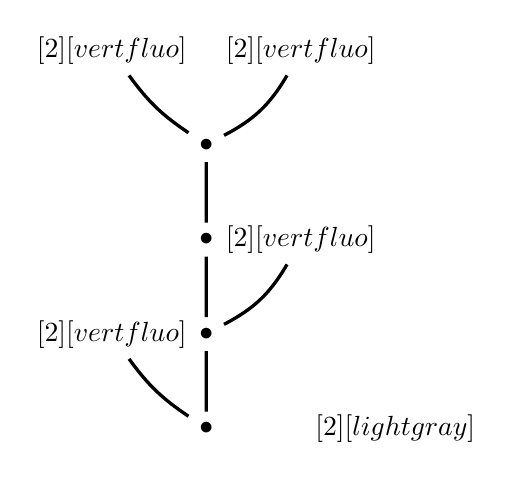
\begin{tikzpicture}[very thick, scale=0.6]

\node (foot) at (2,0) {$\bullet$};
\node (N1) at (2,2) {$\bullet$};
\node (N2) at (2,4) {$\bullet$};
\node (N3) at (2,6) {$\bullet$};
\node (H0) at (0,2) {$\Smiley[2][vertfluo]$};
\node (H1) at (0,8) {$\Smiley[2][vertfluo]$};
\node (H2) at (4,8) {$\Smiley[2][vertfluo]$};
\node (H5) at (4,4) {$\Smiley[2][vertfluo]$};
\node (H4) at (6,0) {$\Xey[2][lightgray]$};
\draw (foot) -- (N1)[very thick] ;
\draw (N1) -- (N2);
\draw (N2) -- (N3) ;
\draw (N3) to [bend left= 10]  (H1) ;
\draw (N3) to [bend right= 16] (H2);
\draw (foot) to [bend left= 10]  (H0) ;
\draw (N1) to [bend right= 16] (H5);
\end{tikzpicture}

\caption{Hy': the state  of Hy after one round \label{fig:Hy-prime}}
\end{figure}


\begin{figure}[hp]
\centering
\begin{tikzpicture}[very thick, scale=0.5]

\node (foot) at (2,0) {$\bullet$};
\node (N1) at (2,2) {$\bullet$};
\node (N2) at (2,4)  {{\color{lightred}$\bullet$}};
\node (N3) at (2,6) {{\color{lightred}$\bullet$}};
\node (H0) at (0,2) {$\Smiley[2][vertfluo]$};
\node (H1) at (0,8) {$\Sey[2][lightred]$};
\node (H2) at (5,0) {$\Xey[2][lightgray]$};
\node (H5) at (4,4) {$\Smiley[2][vertfluo]$};
\node (ex) at (5,8) {};
\draw (foot) -- (N1)[very thick] ;
\draw (N1) -- (N2);
\draw  (N2) -- (N3)[draw=lightred];
\draw (N3) to   [bend left= 10](H1) [draw=lightred];
\draw [dashed] (N3) to [bend left= 10](ex);
\draw (foot) to [bend left= 10]  (H0) ;
\draw (N1) to [bend right= 16] (H5);
\end{tikzpicture}
\caption{A second beheading}
\label{fig:Hy2}
\end{figure}

\begin{figure}[hp]
\centering
\begin{tikzpicture}[very thick, scale=0.6]

\node (foot) at (2,0) {$\bullet$};
\node (N1) at (2,2) {$\bullet$};
\node (N2) at (2,4) {$\bullet$};
\node (N3) at (2,6) {{\color{lightred}$\bullet$}};
\node (H1) at (0,8) {$\Smiley[2][vertfluo]$};
\node (H11) at (2,8) {$\Smiley[2][vertfluo]$};
\node (H12) at (4,8) {$\Smiley[2][vertfluo]$};
\node (H13) at (6,8) {$\Smiley[2][vertfluo]$};
\node (H14) at (8,8) {$\Smiley[2][vertfluo]$};

\node (N3) at (1,6) {$\bullet$};
\node (N31) at (2,6) {$\bullet$};
\node (N32) at (3,6) {$\bullet$};
\node (N33) at (4,6) {$\bullet$};
\node (N34) at (5,6) {$\bullet$};

\node (H0) at (0,2) {$\Smiley[2][vertfluo]$};
\node (H5) at (4,4) {$\Smiley[2][vertfluo]$};
\draw (foot) -- (N1)[very thick] ;
\draw (N1) -- (N2);
\draw (N2) -- (N3);
\draw (N2) -- (N31);
\draw (N2) -- (N32);
\draw (N2) -- (N33);
\draw (N2) -- (N34);
\draw (N3) to   [bend left= 10](H1) ;
\draw (N31) to   [bend left= 10](H11) ;
\draw (N32) to   [bend left= 10](H12) ;
\draw (N33) to   [bend left= 10](H13) ;
\draw (N34) to   [bend left= 10](H14) ;
\draw (foot) to [bend left= 10]  (H0) ;
\draw (N1) to [bend left= 10]  (H5) ;
\end{tikzpicture}
\caption{Hy'', the state of Hy after two rounds \label{fig:Hy3}}
\end{figure}

Figs.~\ref{fig:Hy4} and~\vref{fig:Hy5} represent a possible third round of the battle, with a replication factor equal to $2$. Let us call \texttt{Hy'''} the state of the hydra after that third round.

\begin{figure}[hp]
\centering
\begin{tikzpicture}[very thick, scale=0.6]

\node (foot) at (2,0)  {{\color{lightred}$\bullet$}};
\node (N1) at (2,2) {{\color{lightred}$\bullet$}};
\node (N2) at (2,4) {{\color{lightred}$\bullet$}};
\node (N3) at (2,6) {{\color{lightred}$\bullet$}};
\node (exN4) at (4,4) {};
\node (H1) at (0,8) {$\Sey[2][lightred]$};
\node (H11) at (2,8) {$\Sey[2][lightred]$};
\node (H12) at (4,8) {$\Sey[2][lightred]$};
\node (H13) at (6,8) {$\Sey[2][lightred]$};
\node (H14) at (8,8) {$\Sey[2][lightred]$};

\node (N3) at (1,6) {{\color{lightred}$\bullet$}};
\node (N31) at (2,6) {{\color{lightred}$\bullet$}};
\node (N32) at (3,6) {{\color{lightred}$\bullet$}};
\node (N33) at (4,6) {{\color{lightred}$\bullet$}};
\node (N34) at (5,6) {{\color{lightred}$\bullet$}};

\node (H0) at (0,2) {$\Smiley[2][vertfluo]$};
\node (H5) at (4,0) {$\Xey[2][lightgray]$};
\draw (foot) -- (N1)[very thick,draw=lightred] ;
\draw (N1) -- (N2)[draw=lightred];
\draw (N2) -- (N3)[draw=lightred];
\draw (N2) -- (N31)[draw=lightred];
\draw (N2) -- (N32)[draw=lightred];
\draw (N2) -- (N33)[draw=lightred];
\draw (N2) -- (N34)[draw=lightred];
\draw (N3) to   [bend left= 10](H1) [draw=lightred];
\draw (N31) to   [bend left= 10](H11) [draw=lightred];
\draw (N32) to   [bend left= 10](H12) [draw=lightred];
\draw (N33) to   [bend left= 10](H13) [draw=lightred];
\draw (N34) to   [bend left= 10](H14) [draw=lightred];
\draw (foot) to [bend left= 10]  (H0) ;
\draw [dashed] (N1) to  [bend left= 10](exN4);
\end{tikzpicture}
\caption{A third beheading (wounded part in red) \label{fig:Hy4}}
\end{figure}

\begin{figure}[hp]
\centering
\begin{tikzpicture}[very thick, scale=0.4]

\node (foot) at (10,0) {$\bullet$};


\node (N1) at (2,2) {$\bullet$};
\node (N2) at (2,4) {$\bullet$};
\node (N3) at (2,6) {{\color{lightred}$\bullet$}};
\node (H1) at (0,8) {$\Smiley[1][vertfluo]$};
\node (H11) at (2,8) {$\Smiley[1][vertfluo]$};
\node (H12) at (4,8) {$\Smiley[1][vertfluo]$};
\node (H13) at (6,8) {$\Smiley[1][vertfluo]$};
\node (H14) at (8,8) {$\Smiley[1][vertfluo]$};

\node (N3) at (1,6) {$\bullet$};
\node (N31) at (2,6) {$\bullet$};
\node (N32) at (3,6) {$\bullet$};
\node (N33) at (4,6) {$\bullet$};
\node (N34) at (5,6) {$\bullet$};

\node (H0) at (-3,3) {$\Smiley[1][vertfluo]$};

\draw (foot) to [bend left=10] (N1)[very thick] ;
\draw (N1) -- (N2);
\draw (N2) -- (N3);
\draw (N2) -- (N31);
\draw (N2) -- (N32);
\draw (N2) -- (N33);
\draw (N2) -- (N34);
\draw (N3) to   [bend left= 10](H1) ;
\draw (N31) to   [bend left= 10](H11) ;
\draw (N32) to   [bend left= 10](H12) ;
\draw (N33) to   [bend left= 10](H13) ;
\draw (N34) to   [bend left= 10](H14) ;
\draw (foot) to [bend left = 15]  (H0) ;


% second copy 
\node (N01) at (12,2) {$\bullet$};
\node (N02) at (12,4) {$\bullet$};
\node (N03) at (12,6) {{\color{lightred}$\bullet$}};
\node (H001) at (10,8) {$\Smiley[1][vertfluo]$};
\node (H0011) at (12,8) {$\Smiley[1][vertfluo]$};
\node (H0012) at (14,8) {$\Smiley[1][vertfluo]$};
\node (H0013) at (16,8) {$\Smiley[1][vertfluo]$};
\node (H0014) at (18,8) {$\Smiley[1][vertfluo]$};

\node (N03) at (11,6) {$\bullet$};
\node (N031) at (12,6) {$\bullet$};
\node (N032) at (13,6) {$\bullet$};
\node (N033) at (14,6) {$\bullet$};
\node (N034) at (15,6) {$\bullet$};

\draw (foot) -- (N01)[very thick] ;
\draw (N01) -- (N02);
\draw (N02) -- (N03);
\draw (N02) -- (N031);
\draw (N02) -- (N032);
\draw (N02) -- (N033);
\draw (N02) -- (N034);
\draw (N03) to   [bend left= 10](H001) ;
\draw (N031) to   [bend left= 10](H0011) ;
\draw (N032) to   [bend left= 10](H0012) ;
\draw (N033) to   [bend left= 10](H0013) ;
\draw (N034) to   [bend left= 10](H0014) ;

% third copy 
\node (N001) at (22,2) {$\bullet$};
\node (N002) at (22,4) {$\bullet$};
\node (N003) at (22,6) {{\color{lightred}$\bullet$}};
\node (H001) at (20,8) {$\Smiley[1][vertfluo]$};
\node (H0011) at (22,8) {$\Smiley[1][vertfluo]$};
\node (H0012) at (24,8) {$\Smiley[1][vertfluo]$};
\node (H0013) at (26,8) {$\Smiley[1][vertfluo]$};
\node (H0014) at (28,8) {$\Smiley[1][vertfluo]$};

\node (N003) at (21,6) {$\bullet$};
\node (N0031) at (22,6) {$\bullet$};
\node (N0032) at (23,6) {$\bullet$};
\node (N0033) at (24,6) {$\bullet$};
\node (N0034) at (25,6) {$\bullet$};

\draw (foot) -- (N001)[very thick] ;
\draw (N001) -- (N002);
\draw (N002) -- (N003);
\draw (N002) -- (N0031);
\draw (N002) -- (N0032);
\draw (N002) -- (N0033);
\draw (N002) -- (N0034);
\draw (N003) to   [bend left= 10](H001) ;
\draw (N0031) to   [bend left= 10](H0011) ;
\draw (N0032) to   [bend left= 10](H0012) ;
\draw (N0033) to   [bend left= 10](H0013) ;
\draw (N0034) to   [bend left= 10](H0014) ;
\end{tikzpicture}
\caption{The configuration Hy''' of Hy \label{fig:Hy5}}
\end{figure}
\FloatBarrier

We leave it to the reader  to guess the following  rounds of the battle \dots
 % Please keep in mind that, in this 
% the hydra is free to chose any number of replications at each time, whereas
% Hercules chops only one head per round.

% Let us precise that, in this game, Hercules wins if the hydra is eventually reduced 
% to a single head. 
% We know from~\cite{KP82} that, whichever the initial configuration of the
% hydra, and the strategies of both players, Hercules eventually wins. The 
% aforementionned paper shows also that there do not exist any \emph{simple} proof of this result.


\section{Hydras and their representation in \emph{Coq}}
\label{sec:orgheadline48}


In order to describe trees where each node can have an arbitrary (but finite) number of sons, it usual to define a type where each node carries a \emph{forest}, \emph{i.e} a list of trees
(see for instance Chapter 14, pages 400-406 of \cite{BC04}).

For this purpose, we define two mutual \emph{ad-hoc}  inductive types, where \texttt{Hydra} is the main type, and \texttt{Hydrae} is a helper for describing finite sequences of hydra.
\index{Types!Hydra}

\vspace{4pt}
\emph{From Module~\href{../src/html/hydras.Hydra.Hydra_Definitions.html\#Hydra}{Hydra.Hydra\_Definitions}}

\begin{Coqsrc}
Inductive Hydra : Set :=
|  node :  Hydrae -> Hydra
with Hydrae : Set :=
| hnil : Hydrae
| hcons : Hydra -> Hydrae -> Hydrae.
\end{Coqsrc}

\index{To do}

\begin{todo}
Look for an existing library on trees with nodes of arbitrary arity, iin order to replace  this ad-hoc type with something more generic.
\end{todo}


\index{Projects}

\begin{project}[**]

 Another very similar representation could use the \texttt{list} type family instead of the specific 
type \texttt{Hydrae}:


\begin{Coqalt}
Module Alt.

Inductive Hydra: Set :=
  hnode (daughters : list Hydra).

End Alt.
\end{Coqalt}

Using this representation, re-define all the constructions of this chapter.
You will probably have to use patterns described for instance in~\cite{BC04} or the archives of the Coq-club~\cite{Coq}.

  
\end{project}


\index{Projects}

\begin{project}
The type \texttt{Hydra} above describes hydras as \emph{plane trees}, i.e., as drawn on a sheet of paper or computer screen. Thus, hydras are \emph{oriented},
and it is appropriate to consider a \emph{leftmost} or \emph{rightmost} head of
the beast. It could be interesting to consider another representation, in which
every non-leaf node has a \emph{multi-set} -- not an ordered list -- of daughters.
\end{project}

\subsubsection{Abbreviations}

We provide several notations for ``patterns'' which occur often in our developments. 

\emph{From Module~\href{../src/html/hydras.Hydra.Hydra_Definitions.html\#head}{Hydra.Hydra\_Definitions}}

\begin{Coqsrc}
(** heads *)
Notation head := (node hnil).
 
(** nodes  with 1, 2 or 3 daughters *)
Notation hyd1 h := (node (hcons h hnil)).
Notation hyd2 h h' := (node (hcons h (hcons h' hnil))).
Notation hyd3 h h' h'' := 
                   (node (hcons h (hcons h' (hcons h'' hnil)))).
\end{Coqsrc}


For instance, the hydra \texttt{Hy}  of Figure~\vref{fig:Hy} is defined in \emph{Gallina} as follows:

\vspace{4mm}
\emph{From Module~\href{../src/html/hydras.Hydra.Hydra_Examples.html\#Hy}{Hydra.Hydra\_Examples}}

\begin{Coqsrc}
Example Hy := hyd3 head
                   (hyd2
                      (hyd1 
                         (hyd2 head head))
                      head) 
                   head.
\end{Coqsrc}



Hydras quite frequently contain  multiple  copies of the same pattern. The following functions
will help us to describe and reason about replications in hydra battles.

\vspace{4pt}

\emph{From Module~\href{../src/html/hydras.Hydra.Hydra_Definitions.html\#hcons_mult}{Hydra.Hydra\_Definitions}}

\begin{Coqsrc}
Fixpoint hcons_mult (h:Hydra)(n:nat)(s:Hydrae):Hydrae :=
  match n with 
  | O => s
  | S p => hcons h (hcons_mult h p s)
  end.

(** hydra with n copies of the same daughter *)

Definition hyd_mult h n :=
  node (hcons_mult h n hnil).
\end{Coqsrc}

\vspace{4mm}



For instance, the hydra $Hy''$ of Fig~\vref{fig:Hy3}  can be defined in \coq{} as follows:

\vspace{4pt}

\emph{From Module~\href{../src/html/hydras.Hydra.Hydra_Examples.html}{Hydra.Hydra\_Examples}}

\begin{Coqsrc}
Example Hy'' := 
     hyd2 head
          (hyd2 (hyd_mult (hyd1 head) 5)
                head).
\end{Coqsrc}




\subsubsection{Recursive functions on type \texttt{Hydra}}
\label{sec:orgheadline41}
\label{sec:hsize-def}




When defining a recursive function over the type \texttt{Hydra}, one has to consider the three constructors 
\texttt{node}, \texttt{hnil} and \texttt{hcons} of the mutually inductive types \texttt{Hydra} and \texttt{Hydrae}. 
Let us define for instance the function that  computes the number of nodes of any hydra:

\vspace{4pt}
\emph{From Module~\href{../src/html/hydras.Hydra.Hydra_Definitions.html}{Hydra.Hydra\_Definitions}}


\begin{Coqsrc}
Fixpoint hsize (h:Hydra) : nat :=
  match h with node l => S (lhsize l)
  end
with lhsize l : nat :=
  match l with hnil => 0
            | hcons h hs => hsize h + lhsize hs 
  end.

 Compute hsize Hy.
\end{Coqsrc}

\begin{Coqanswer}
 = 9
     : nat 
\end{Coqanswer}


Likewise, the \emph{height} (maximum distance between the foot and a head) 
is defined by mutual recursion:

\begin{Coqsrc}
Fixpoint height  (h:Hydra) : nat :=
  match h with node l => lheight l
  end
with lheight l : nat :=
  match l with 
  | hnil => 0
  | hcons h hs => Max.max (S (height h)) (lheight hs)
  end.
\end{Coqsrc}

\begin{Coqsrc}
Compute height Hy.
\end{Coqsrc}

\begin{Coqanswer}
 = 4
     : nat  
\end{Coqanswer}

\index{Exercises}

\begin{exercise}
Define a function \texttt{max\_degree: Hydra $\arrow$ nat} which  returns the highest degree of a node in any hydra. For instance, the evaluation of the term \texttt{(max\_degree Hy)} should return $3$.
\end{exercise}

\subsection{Induction principles for hydras}
\label{sec:orgheadline42}


In this section, we show how induction principles are used to prove properties on the type 
\texttt{Hydra}. Let us consider for instance the following statement:
\begin{quote}
  `` The height of any hydra is strictly less than its size. ''
\end{quote}



\subsubsection{A failed attempt}

One may try to use the default tactic of proof by induction, that corresponds to an application of the automatically  generated  induction principle for  type \texttt{Hydra}:

\begin{Coqanswer}
Hydra_ind :
forall P : Hydra -> Prop,
(forall h : Hydrae, P (node h)) -> forall h : Hydra, P h
\end{Coqanswer}

Ler us start a simple proof by induction.

\vspace{4pt}
\emph{From Module~\href{../src/html/hydras.Hydra.Hydra_Examples.html}{Hydra.Hydra\_Examples}}

\begin{Coqbad}
Module Bad.

Lemma height_lt_size (h:Hydra) :
  height h <= hsize h.
Proof.
  induction h as [s].
\end{Coqbad}

\begin{Coqanswer}
1 subgoal, subgoal 1 (ID 11)
  
  s : Hydrae
  ============================
   height (node s) <= hsize (node s)
\end{Coqanswer}

We might be tempted to do an induction on the sequence \texttt{s}:

% \begin{Coqbad}
% induction  s as [ | h s'].
%   -   cbn; auto with arith.
%   - 
% \end{Coqbad}


\begin{Coqanswer}
 1 focused subgoal
(unfocused: 0), subgoal 1 (ID 19)
  
  h : Hydra
  s' : Hydrae
  IHs' : height (node s') <= hsize (node s')
  ============================
   height (node (hcons h s')) <= hsize (node (hcons h s'))

\end{Coqanswer}

Note that the displayed subgoal does not contain any assumption on \texttt{h}, thus there is no way to 
infer any property about the height and size of the hydra \texttt{(hcons h t)}.

\begin{Coqbad}
Abort.

End Bad.
\end{Coqbad}

\subsubsection{A principle for  mutual induction}
In order to get an appropriate induction scheme for the types 
\texttt{Hydra} and \texttt{Hydrae}, we can use  \coq{}'s  command \texttt{Scheme}.


\index{Coq!Techniques!Mutual induction}
\index{Coq!Commands!Scheme}

\begin{Coqsrc}
Scheme Hydra_rect2 := Induction for Hydra Sort Type
with Hydrae_rect2 := Induction for Hydrae Sort Type.
\end{Coqsrc}  


\begin{Coqsrc}
Check Hydra_rect2.
\end{Coqsrc}


\begin{Coqanswer}
Hydra_rect2
 : forall (P : Hydra -> Type) (P0 : Hydrae -> Type),
   (forall h : Hydrae, P0 h -> P (node h)) ->
    P0 hnil ->
    (forall h : Hydra, P h -> 
             forall h0 : Hydrae, P0 h0 -> P0 (hcons h h0)) ->
    forall h : Hydra, P h
\end{Coqanswer}  




\subsubsection{A correct proof}

Let us now use \texttt{Hydra\_rect2} for proving that the height of any hydra is strictly less than its size.
Using this scheme requires an auxiliary predicate, called \texttt{P0} in \texttt{Hydra\_rect2}'s statement. 
Let us begin by defining an ad-hoc version of \texttt{List.Forall}.

\vspace{4pt}
\emph{From Module~\href{../src/html/hydras.Hydra.Hydra_Examples.html}{Hydra.Hydra\_Examples}}

\begin{Coqsrc}
(** All elements of s satisfy P *)

Fixpoint h_forall (P: Hydra -> Prop) (s: Hydrae) :=
  match s with
      hnil => True
    | hcons h s' => P h /\ h_forall P s'
  end.
 \end{Coqsrc}

 \begin{Coqsrc}
Lemma height_lt_size (h:Hydra) :
 height h < hsize h.
Proof.
  induction h using Hydra_rect2  with 
  (P0 :=  h_forall (fun h =>  height h < hsize h)).
 \end{Coqsrc}

\begin{enumerate}
\item The first subgoal is as follows:

\begin{Coqanswer}

  h: Hydrae
  IHh : h_forall (fun h : Hydra => height h < hsize h) h
  ============================
   height (node s) < hsize (node s) 

\end{Coqanswer}

This goal is easily solvable, using some arithmetic. We let the reader look at the source of this development.

\item The second subgoal is trivial:

\begin{Coqanswer}

  ============================
    h_forall (fun h : Hydra => height h < hsize h) hnil

\end{Coqanswer}

\begin{Coqsrc}
  reflexivity.
\end{Coqsrc}

\item Finally, the last subgoal is also easy to solve:



\begin{Coqanswer}
  h : Hydra
  h0 : Hydrae
  IHh : height h < hsize h
  IHh0 : h_forall (fun h : Hydra => height h < hsize h) h0
  ============================
   h_forall (fun h1 : Hydra => height h1 < hsize h1) 
                 (hcons h h0)
\end{Coqanswer}  



\begin{Coqsrc}
 split;auto. 
Qed.   
\end{Coqsrc}

\end{enumerate}

\index{Exercises}

\begin{exercise}
It happens very often that, in the proof of  a proposition of the form 
(\texttt{$\forall\,$ h:Hydra, $P$ h}), the predicate \texttt{P0}
is  (\texttt{h\_forall $P$}).  Design a tactic for induction on hydras that frees the user from binding explicitly \texttt{P0},  and solves trivial subgoals. Apply it for writing  a shorter proof of \texttt{height\_lt\_size}.
\end{exercise}
 


\section{Relational description of hydra battles}


In this section, we represent the rules of hydra battles as a binary relation associated with
a \emph{round}, i.e., an interaction composed of the two following actions:
\begin{enumerate}
\item Hercules chops off one head of the hydra
\item Then, the  hydra replicates the wounded part (if the head is at distance $\geq 2$ from the foot).
\end{enumerate}
The relation associated with each round of the battle is \emph{parameterized}  by the \emph{expected} replication  factor (irrelevant if the chopped head is at distance 1 from the foot,
but present for consistency's sake).

In our description,  we will apply the following naming convention: if $h$ represents the configuration of the hydra before a round, then the configuration of $h$ after this round will be called $h'$.
 Thus, we are going to define a proposition  (\texttt{round\_n $n\;h\;h'$})  whose intended meaning will be `` the hydra $h$  is transformed into $h'$  in a single round of a battle, with the expected replication factor $n$ ''.


Since the replication of parts of the hydra depends on the distance of the chopped head from  the foot, we  decompose our description into two main  cases, under the form of a bunch of [mutually] inductive predicates over the types \texttt{Hydra} and \texttt{Hydrae}.

The mutually exclusive cases we consider are the following.
\begin{itemize}
\item \textbf{R1}: The chopped off head was at distance 1 from the foot.
\item \textbf{R2}: The chopped off head was at a distance greater than or equal to  $2$ from the foot.
\end{itemize}



\subsection{Chopping off a head at distance 1 from the foot (relation  R1)}

If Hercules chops off a head near the floor, there is no replication at all. We use an auxiliary predicate, associated with the removing of one head from a sequence of hydras.

\pagebreak
\vspace{4pt}\emph{From Module\href{../src/html/hydras.Hydra.Hydra_Definitions.html}{Hydra.Hydra\_Definitions}}

\begin{Coqsrc}
Inductive S0 :  relation Hydrae :=
| S0_first : forall s, S0  (hcons head s) s
| S0_rest : forall  h s s',  S0  s s' ->
                             S0  (hcons h s) (hcons h s').

Inductive R1  :  Hydra -> Hydra -> Prop :=
| R1_intro : forall s s', S0 s s' -> R1 (node s) (node s').
\end{Coqsrc}

\subsubsection{Example}
\label{sec:orgheadline45}

Let us represent in \coq{}   the transformation of the hydra of Fig.~\vref{fig:Hy} into
the configuration represented in Fig.~\ref{fig:Hy-prime}.

\vspace{4pt}
\emph{From Module~\href{../src/html/hydras.Hydra.Hydra_Examples.html}{Hydra.Hydra\_Examples}}


\begin{Coqsrc}
Example Hy_1 : R1 Hy Hy'.
Proof. 
  split; right; right; left.
Qed.
\end{Coqsrc}


\subsection{Chopping of a head at distance \texorpdfstring{$\geq 2$}{>= 2} from the foot (relation R2) }


Let us now consider beheadings  where the chopped-off head is at distance greater than or equal to $2$ from the foot. All the following relations are parameterized by the number $n$ of new copies added by the hydra.

 Let $s$ be a sequence of hydras. 
The proposition (\texttt{S1 n s s'}) holds if $s'$ is obtained by replacing some element $h$ of $s$ by 
$n+1$ copies of $h'$, where  the proposition (\texttt{R1 h h'}) holds, in other words, \texttt{h'} is just \texttt{h}, without the chopped-off  head. \texttt{S1} is an inductive relation with two constructors that allow us to choose the position in $s'$ of the wounded sub-hydra $h$.

\vspace{4pt}
\emph{From Module~\href{../src/html/hydras.Hydra.Hydra_Definitions.html\#S1}{Hydra.Hydra\_Definitions}}

\begin{Coqsrc}
Inductive S1 (n:nat)  : Hydrae -> Hydrae -> Prop :=
| S1_first : forall s h h' ,   R1 h h' -> 
                  S1 n (hcons h s) (hcons_mult h' (S n) s)
| S1_next : forall h s s',  S1 n s s' ->
                   S1 n (hcons h s) (hcons h s').
\end{Coqsrc}


The rest of the definition is structured as two mutually inductive relations on hydras and sequences of hydras. The first constructor of \texttt{R2} describes the case where the chopped head is exactly at height $2$. The others constructors allow us to consider beheadings at height strictly greater than $2$.


\vspace{4pt}
\emph{From Module~\href{../src/html/hydras.Hydra.Hydra_Definitions.html\#R2}{Hydra.Hydra\_Definitions}}

\begin{Coqsrc}
Inductive R2 (n:nat)  :  Hydra -> Hydra -> Prop :=
| R2_intro : forall s s', S1 n s s' -> R2 n (node s) (node s')
| R2_intro_2 : forall s s', S2 n s s' -> R2 n (node s) (node s')

with S2 (n:nat) :  Hydrae -> Hydrae -> Prop :=
|  S2_first : forall h h' s ,
               R2 n  h h'  -> 
               S2  n (hcons h s) (hcons h'  s)
|  S2_next  : forall h   r r',
               S2 n   r r' ->
               S2 n (hcons h r) (hcons h r').                  
\end{Coqsrc}


\subsubsection{Example}
Let us prove the transformation of \texttt{Hy'} into \texttt{Hy''} (see Fig.~\vref{fig:Hy3}).

\vspace{4pt}\emph{From Module~\href{../src/html/hydras.Hydra.Hydra_Examples.html}{Hydra.Hydra\_Examples}}. 

\begin{Coqsrc}
Example R2_example:  R2 4 Hy' Hy''.
Proof.
  right. right. left.  right. left. left. left. split. left.
Qed.
\end{Coqsrc}

The reader is encouraged to look at all the intermediary subgoals of this example.
\emph{Please consider also exercise~\vref{exo:interactive-battle}.}


\subsection{Description of any round}

We combine the two cases above into a single relation.
First,  we define the  relation \texttt{(round\_n n h h')} where \texttt{n} is the expected number of  replications (irrelevant in the case of an \texttt{R1}-transformation).

\vspace{4pt}
\emph{From Module~\href{../src/html/hydras.Hydra.Hydra_Definitions.html\#round_n}{Hydra.Hydra\_Definitions}}

\index{Predicates!round\_n}

\begin{Coqsrc}
Definition round_n n h h' := R1 h h' \/ R2 n h h'.  
\end{Coqsrc}

By abstraction over \texttt{n}, we define a \emph{round} (small step) of a battle:

\index{Predicates!round}

\begin{Coqsrc}
Definition round h h' := exists n,  round_n n h h'.

Infix "-1->" := round (at level 60).
\end{Coqsrc}

\index{Projects}

\begin{project}
Give a direct translation of Kirby and Paris's description of hydra battles (quoted on page~\pageref{original-rules}) and prove that our relational description is consistent with theirs.
\end{project}


\subsection{Rounds and battles}


Using library \href{https://coq.inria.fr/distrib/current/stdlib/Coq.Relations.Relation_Operators.html}{Relations.Relation\_Operators}, we define \texttt{round\_plus},  the transitive closure of \texttt{round}, and \texttt{round\_star},  the reflexive and transitive closure of \texttt{round}.


\begin{Coqsrc}
Definition round_plus := clos_trans_1n Hydra round.
Infix "-+->" := rounds (at level 60).

Definition round_star h h' := h = h' \/ round_plus h h'.
Infix "-*->" := round_star (at level 60).
\end{Coqsrc}

\index{Notations!''-+->''}
\index{Notations!''-*->''}

\index{Exercises}

\begin{exercise}
Prove the following lemma:

\begin{Coqsrc}
Lemma rounds_height : forall h h', 
   h -+-> h' -> height h' <= height h.  
\end{Coqsrc}
  
\end{exercise}

\begin{remark}
\coq's library \href{https://coq.inria.fr/distrib/current/stdlib/Coq.Relations.Relation_Operators.html}{Coq.Relations.Relation\_Operators} 
contains three logically equivalent definitions of the transitive closure of a binary relation. This equivalence is proved in 
\href{https://coq.inria.fr/distrib/current/stdlib/Coq.Relations.Operators_Properties.html}{Coq.Relations.Operators\_Properties} . 

Why three definitions for a single mathematical concept?
Each definition generates an associated induction principle. 
 According to the form of statement one would like to prove, there is a ``best choice'':

\begin{itemize}
\item For proving $\forall y, x\,R^+\,y \;\arrow\; P\,y$, prefer 
\texttt{clos\_trans\_n1}
\item For proving $\forall x,\,x\,R^+\,y \;\arrow\; P\,x$, prefer \texttt{clos\_trans\_1n}
\item For proving $\forall x\,y, \,x\,R^+\,y \;\arrow\;P\,x\,y$,  
prefer \texttt{clos\_trans},
\end{itemize}
But there is no ``wrong choice'' at all: the equivalence lemmas in \linebreak 
\href{https://coq.inria.fr/distrib/current/stdlib/Coq.Relations.Operators_Properties.html}{Coq.Relations.Operators\_Properties} 
 allow the user
to convert any one of the three closures into another one before applying the corresponding elimination tactic.
The same remark also holds for reflexive and transitive closures. 
\end{remark}

\index{Exercises}

\begin{exercise}
Define a restriction of \coqsimple{round},  where Hercules always chops off
the leftmost among the lowest heads.

Prove that, if $h$ is not a simple head, then there exists a unique $h'$ such that \texttt{h}  is transformed into \texttt{ h'} in one round, according to this restriction.


\end{exercise}

\index{Exercises}

\begin{exercise}[Interactive battles]
\label{exo:interactive-battle}
Given a hydra \texttt{h}, the specification of a hydra battle for \texttt{h} is the type 
\Verb@{h':Hydra | h -*-> h'}@. In order to avoid long sequences of \texttt{split}, \texttt{left}, and 
\texttt{right}, design a set of dedicated tactics for the interactive building of a battle.
Your tactics will have the following functionalities:
\begin{itemize}
\item  Chose to stop a battle, or continue
\item Chose an expected number of replications
\item Navigate in a hydra, looking for a head to chop off.
\end{itemize}

Use your tactics for simulating a small part of a hydra battle, for instance the rounds which lead from
\texttt{Hy} to \texttt{Hy'''}  (Fig.~\vref{fig:Hy5}).

\textbf{Hint:} Please keep in mind that the last  configuration of your interactively built battle is known only at the end of the battle. Thus, you will have to create and solve subgoals with existential variables. For that purpose, the tactic \texttt{eexists}, applied to the 
goal \Verb@{h':Hydra | h -*-> h'}@ generates the subgoal \Verb|h -*-> ?h'|.
\end{exercise}


\subsection{Classes of battles}
\label{sect:battle-classes}

In some presentations of hydra battles, e.g.~\cite{KP82, bauer2008}, the transformation associated with the $i$-th round may depend on $i$. For instance, in these articles, the replication factor at the $i$-th round is equal to $i$. In other examples, one can allow the hydra to apply any replication factor at any time. In order to be the most general as possible, we define the type of predicates which relate the state of the hydra before and after the $i$-th round of a battle.

\vspace{4pt}
\emph{From Module~\href{../src/html/hydras.Hydra.Hydra_Definitions.html}{Hydra.Hydra\_Definitions}}
\index{Coq!Techniques!Type classes}

\begin{Coqsrc}
Definition dep_round_t := nat -> Hydra -> Hydra -> Prop.

Class Battle :=  {battle_r : dep_round_t;
                  battle_inclusion : forall i h h',
                      battle_r i h h' -> round h h'}.

\end{Coqsrc}

The most general class of battles is \texttt{free}, which allows the hydra to chose any replication factor at every step:

\vspace{4pt}
\emph{From Module~\href{../src/html/hydras.Hydra.Hydra_Definitions.html\#free}{Hydra.Hydra\_Definitions}}

\begin{Coqsrc}
Program Instance free : Battle :=
  (Build_Battle ( fun _  h h' => round h h') _).
\end{Coqsrc}

We chosed to call \emph{standard} the kind of battles which appear  most often in the litterature and correspond to an arithmetic progression of the replication factor : $0,1,2,3, \dots$

\vspace{4pt}
\emph{From Module~\href{../src/html/hydras.Hydra.Hydra_Definitions.html\#standard}{Hydra.Hydra\_Definitions}}

\begin{Coqsrc}
Program Instance standard : Battle := (Build_Battle round_n _).
Next Obligation.
  now exists i.  
Defined.
\end{Coqsrc}


\subsection{Big steps}

Let $B$ be any instance of class \texttt{Battle}. It is easy to define inductively the relation between the $i$-th and the $j$-th steps of a battle of type $B$.

\vspace{4pt}
\emph{From Module~\href{../src/html/hydras.Hydra.Hydra_Definitions.html\#fight}{Hydra.Hydra\_Definitions}}

\begin{Coqsrc}
Inductive battle (B:Battle) : nat -> Hydra -> nat -> Hydra -> Prop :=

| battle_1 : forall i h  h', battle_r   B i  h h' -> 
                            battle B i h (S i) h'
| battle_n : forall i h  j h' h'',  battle_r  B i h h''  ->
                                   battle B (S i) h'' j h'  ->
                                   battle B i h j h'.
\end{Coqsrc}

% \begin{remark}
%  The class \texttt{free} is strongly related with the transitive closure  \texttt{round\_plus}, as expressed by the following lemmas.

% \vspace{4pt}
% \emph{From Module~\href{../src/html/hydras.Hydra.Hydra_Lemmas.html}{Hydra.Hydra\_Lemmas}}

%  \begin{Coqsrc}
%  Lemma battle_free_equiv1 : forall i j h h',  
%              battle free i h j h' ->   h -+-> h'.
 
%  Lemma battle_free_equiv2 : forall h h',
%      h -+-> h' ->
%     forall i, exists j,  battle free i h j h'.
%  \end{Coqsrc}

% \end{remark}



\section{A long battle}
\label{sect:big-battle}


In this section we consider a simple example of battle, starting with a small hydra,
shown on figure~\vref{fig:hinit}, with a simple strategy for both players:

\begin{itemize}
\item Hercules chops always the rightmost head of the hydra.
\item The battle is standard: at the round number $i$, the expected replication is $i$.
\end{itemize}



\begin{figure}[h]
  \centering
  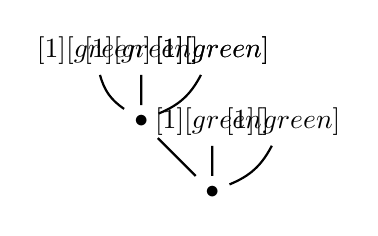
\begin{tikzpicture}[thick, scale=0.30]
 \node (foot) at (6,0) {$\bullet$};
\node (n1) at  (3,3) {$\bullet$};
\node (h1) at  (1,6) {$\Smiley[1][green]$};
\node (h2) at  (3,6) {$\Smiley[1][green]$};
\node (h3) at  (6,6) {$\Smiley[1][green]$};
\node (h4) at  (6,6) {$\Smiley[1][green]$};
\node (h5) at  (6,3) {$\Smiley[1][green]$};
\node (h6) at  (9,3) {$\Smiley[1][green]$};
\draw (foot) -- (n1);
\draw (n1) to   [bend left=20] (h1);
\draw (n1) to   (h2);
\draw (n1) to   [bend right=20] (h3);
\draw (foot) -- (h5);
\draw (foot) to  [bend right=20] (h6);
\end{tikzpicture}

  \caption{The hydra hinit}
  \label{fig:hinit}
\end{figure}


\begin{Coqsrc}
Definition hinit := hyd3 (hyd_mult head 3)  head head.  
\end{Coqsrc}



The lemma we would like to prove is ``The considered battle lasts exactly $N$ rounds'',
with $N$ being a natural number we gave to guess.

But the  battle is so long that no \emph{test} can give us an estimation of its length, and we do need the expressive power of logic to compute this length. However, in order to  guess this length, we made some experiments, computing with \gallina{}, \coq{}'s  functional programming language.
Thus, we can consider this development as a collaboration of proof with computation.

In the following lines, we try to show faithfully how we found the value of the number $N$.

The complete proof is in file \url{../src/html/hydras.Hydra.BigBattle.html}. 

\subsection{The beginning of hostilities}
During the two first rounds, our hydra loses its two rightmost heads. Thus just before the third round, it looks like in figure~\vref{fig:hinit-plus2}.


\begin{figure}[h]
  \centering
  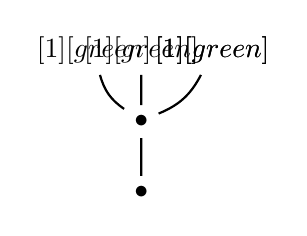
\begin{tikzpicture}[thick, scale=0.30]
 \node (foot) at (3,0) {$\bullet$};
\node (n1) at  (3,3) {$\bullet$};
\node (h1) at  (1,6) {$\Smiley[1][green]$};
\node (h2) at  (3,6) {$\Smiley[1][green]$};
\node (h3) at  (6,6) {$\Smiley[1][green]$};
\node (h4) at  (6,6) {$\Smiley[1][green]$};
\draw (foot) -- (n1);
\draw (n1) to   [bend left=20] (h1);
\draw (n1) to   (h2);
\draw (n1) to   [bend right=20] (h3);
\end{tikzpicture}

  \caption{The hydra (hyd1 h3)}
  \label{fig:hinit-plus2}
\end{figure}

The following lemma  is a formal statement about these first rounds, in terms of the
\texttt{battle} predicate.

\begin{Coqsrc}
Lemma L_0_2 : battle standard 0 hinit 2 (hyd1 h3).   
\end{Coqsrc}


\subsection{Looking for regularities}


A first study with pencil and paper suggested us that, after three rounds, the hydra always looks like in figure~\vref{fig:hinit-plusn} (with a variable number of 
subtrees of height 1 or 0).
Thus, we introduce handy notations.

\begin{Coqsrc}
Notation h3 := (hyd_mult head 3).
Notation h2 := (hyd_mult head 2).
Notation h1 := (hyd1 head).

Definition hyd a b c := 
  node (hcons_mult h2  a
             (hcons_mult h1  b
                         (hcons_mult head c hnil))).
\end{Coqsrc}


For instance Fig~\vref{fig:hinit-plusn} shows the hydra (\texttt{hyd 3 4 2}). The hydra (\texttt{hyd 0 0 0})  is the ``final'' hydra of any terminating battle, {i.e.},
a tree whith exactly one node and no edge.


\begin{figure}[h]
  \centering
  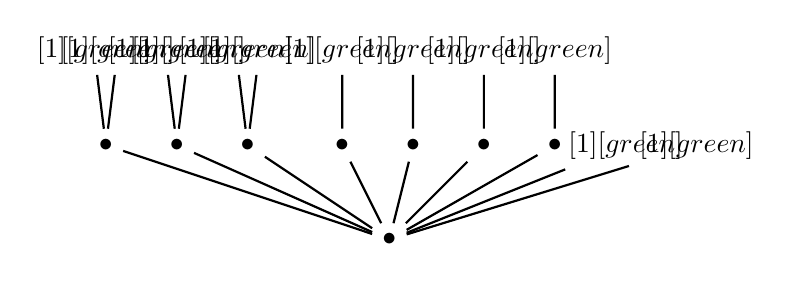
\begin{tikzpicture}[thick, scale=0.30]
 \node (foot) at (15,0) {$\bullet$};
\node (a) at  (3,4) {$\bullet$};
\node (b) at  (6,4) {$\bullet$};
\node (c) at  (9,4) {$\bullet$};
\node (d) at  (13,4) {$\bullet$};
\node (e) at  (16,4) {$\bullet$};
\node (f) at  (19,4) {$\bullet$};
\node (g) at  (22,4) {$\bullet$};
\node (h) at  (25,4) {$\Smiley[1][green]$};
\node (i) at  (28,4) {$\Smiley[1][green]$};
\node (aa) at  (2.5,8) {$\Smiley[1][green]$};
\node (ab) at  (3.5,8) {$\Smiley[1][green]$};
\node (ba) at  (5.5,8) {$\Smiley[1][green]$};
\node (bb) at  (6.5,8) {$\Smiley[1][green]$};
\node (ca) at  (8.5,8) {$\Smiley[1][green]$};
\node (cb) at  (9.5,8) {$\Smiley[1][green]$};
\node (da) at  (13,8) {$\Smiley[1][green]$};
\node (ea) at  (16,8) {$\Smiley[1][green]$};
\node (fa) at  (19,8) {$\Smiley[1][green]$};
\node (ga) at  (22,8) {$\Smiley[1][green]$};
\draw (foot) -- (a);
\draw (foot) -- (b);
\draw (foot) -- (c);
\draw (foot) -- (d);
\draw (foot) -- (e);
\draw (foot) -- (f);
\draw (foot) -- (g);
\draw (foot) -- (h);
\draw (foot) -- (i);
\draw (a) -- (aa);
\draw (a) -- (ab);
\draw (b) -- (ba);
\draw (b) -- (bb);
\draw (c) -- (ca);
\draw (c) -- (cb);
\draw (d) -- (da);
\draw (e) -- (ea);
\draw (f) -- (fa);
\draw (g) -- (ga);
% \node (a) at  (3,4) {$\bullet$};
% \node (h1) at  (1,6) 
% \node (h2) at  (3,6) {$\Smiley[1][green]$};
% \node (h3) at  (6,6) {$\Smiley[1][green]$};
% \node (h4) at  (6,6) {$\Smiley[1][green]$};
% \draw (foot) -- (n1);
% \draw (n1) to   [bend left=20] (h1);
% \draw (n1) to   (h2);
% \draw (n1) to   [bend right=20] (h3);
\end{tikzpicture}

  \caption{The hydra (hyd 3 4 2)}
  \label{fig:hinit-plusn}
\end{figure}


With these notations, we get a formal description of the first three rounds.


\begin{Coqsrc}
Lemma L_2_3 : battle standard 2 (hyd1 h3)  3 (hyd 3 0 0).

Lemma L_0_3 : battle standard 0 hinit 3 (hyd 3 0 0).
\end{Coqsrc}


\subsection{Computing \dots}
In order to study \emph{experimentally} the different  configurations of the  battle, we will use a simple datatype for representing the states as tuples composed of
the round number, and the respective number of daughters  \texttt{h2}, \texttt{h1}, and heads
of the current hydra.




\begin{Coqsrc}
 Record state : Type :=
    mks {round: nat ; n2 : nat ; n1 : nat ; nh : nat}.
\end{Coqsrc}

The following function returns the next configurarion of the game. 
Note that this function is defined only for making experiments and is not  ``certified''.  Formal proofs about our battle will only start with the lemma
\texttt{lemma:step-battle}, page~\pageref{lemma:step-battle}.


\begin{Coqsrc}
Definition next (s : state) :=
  match s with
  | mks round a b (S c) => mks (S round) a b c
  | mks round a (S b) 0 => mks (S round) a b (S round)
  | mks round (S a) 0 0 => mks (S round) a (S round) 0
  | _ => s
  end.
\end{Coqsrc}

We can make bigger steps through iterations of \texttt{next}.

\begin{Coqsrc}
Fixpoint iterate {A:Type} (f : A -> A) (n:nat) (x: A) :=
 match n with 
  | 0 => x
  | S p => f (iterate f p x)
 end.
\end{Coqsrc}

The following function computes the state of the battle at the $n$-th round.


\begin{Coqsrc}
Definition test n := iterate next (n-3) (mks 3 3 0 0).

Compute test 3.
   (**
     = {| round := 3; n2 := 3; n1 := 0; nh := 0 |}
     : state
    *)

Compute test 4.
 (*
  = {| round := 4; n2 := 2; n1 := 4; nh := 0 |}
     : state
 *)

Compute test 5.
 (*
   = {| round := 5; n2 := 2; n1 := 3; nh := 5 |}
     : state
 *)

Compute test 2000.
(*
  = {| round := 2000; n2 := 1; n1 := 90; nh := 1102 |}
     : state
*)
\end{Coqsrc}


The battle we study seems to be awfully long. Let us concentrate our
tests on some particular events : the states where $\texttt{nh}=0$ 

From the value of \texttt{test 5},  it is obvious that at the 10-th round, the counter \texttt{nh} will be
equal to zero.

 \begin{Coqsrc}
 Compute test 10.
(*

    = {| round := 10; n2 := 2; n1 := 3; nh := 0 |}
     : state
*)
 \end{Coqsrc}

Thus, $ (1 + 11)$ rounds later, the \texttt{n1} field will be equal to $2$, and 
\texttt{nh}  will equal to $0$. 


\begin{Coqsrc}
Compute test 22.
(*

 = {| round := 22; n2 := 2; n1 := 2; nh := 0 |}
     : state
*)
\end{Coqsrc}


\begin{Coqsrc}
 Compute test 46.
(*

 = {| round := 46; n2 := 2; n1 := 1; nh := 0 |}
     : state

*)

Compute test 94.

(*

 = {| round := 94; n2 := 2; n1 := 0; nh := 0 |}
     : state

*) 
\end{Coqsrc}


Next round, we decrement \texttt{n2} and set \texttt{n1} to $95$.


\begin{Coqsrc}
 Compute test 95.

(*

  = {| round := 95; n2 := 1; n1 := 95; nh := 0 |}
     : state

*)
\end{Coqsrc}

We now have some intuition of the sequence.
It looks like the next ``\texttt{nh}=0'' event will happen at the $192=2(95+1)$-th round, then at the $2(192+1)$-th round.


\begin{Coqsrc}
 Definition doubleS (n : nat) := 2 * (S n).

Compute test (doubleS 95).

(**
 = {| round := 192; n2 := 1; n1 := 94; nh := 0 |}
     : state
 *)


Compute test (iterate doubleS 2 95).

(*
  = {| round := 386; n2 := 1; n1 := 93; nh := 0 |}
     : state
*)
\end{Coqsrc}

\subsection{Proving \dots}
We are now able to reason about the sequence of transitions defined by our hydra battle. Instead of using the data-type \texttt{state} we study the relationship
between different configurations of the battle.

Let us define a binary relation associated with every round of the battle.
In the following definition \texttt{i} is associated with the round number (or date, if we consider a discrete time), and \texttt{a}, \texttt{b}, \texttt{c} respectively associated with the number of \texttt{h2}, \texttt{h1} and heads connected to the hydra's foot.

\begin{Coqsrc}
Inductive one_step (i: nat) :
  nat -> nat -> nat -> nat -> nat -> nat -> Prop :=
| step1 : forall a b c,  one_step i a b (S c) a b c
| step2 : forall a b ,  one_step i a (S b) 0 a b (S i)
| step3  : forall a, one_step i (S a) 0 0 a (S i) 0.
\end{Coqsrc}

The relation between \texttt{one\_step} and the rules of hydra battle is asserted by the following lemma. 

\label{lemma:step-battle}

\begin{Coqsrc}
Lemma step_battle : forall i a b c a' b' c', 
   one_step i a b c a' b' c' ->
   battle standard i (hyd  a b c)  (S i) (hyd a' b' c').
\end{Coqsrc}

Next, we define ``big steps'' as the transitive closure of \texttt{one\_step},
and reachability (from the initial configuration of figure~\ref{fig:hinit} at time $0$).



\begin{Coqsrc}
 Inductive steps : nat -> nat -> nat -> nat ->
                  nat -> nat -> nat -> nat -> Prop :=
| steps1 : forall i a b c a' b' c',
    one_step i a b c a' b' c' -> steps i a b c (S i) a' b' c'
| steps_S : forall i a b c j a' b' c' k a'' b'' c'',
    steps i a b c j a' b' c' ->
    steps j a' b' c' k a'' b'' c'' ->
    steps i a b c k  a'' b'' c''.

Definition reachable (i a b c : nat) : Prop :=
  steps 3 3 0 0 i a b c.
\end{Coqsrc}


The following lemma establishes a relation between \texttt{steps} and the predicate \texttt{battle}.

\begin{Coqsrc}
 Lemma steps_battle : forall i a b c j a' b' c', 
   steps i a b c j a' b' c' ->
   battle standard i (hyd  a b c)   j  (hyd a' b' c').
\end{Coqsrc}

Thus, any result about \texttt{steps} will be applicable to standard battles.
Using the predicate \texttt{steps} our study of the length of the considered battle
can  be decomposed into three parts:

\begin{enumerate}
\item  Characterization of regularities of some events
\item Study of the beginning of the battle
\item Computing the exact length of the battle.
\end{enumerate}

First, we prove that, if at round $i$ the hydra is equal to
(\texttt{hyd a (S b) 0}), then it will be equal to (\texttt{hyd a b 0}) at the $2(i+1)$-th round.  

\begin{Coqsrc}
Lemma LS : forall c a b i,  steps i a b (S c) (i + S c) a b 0.
Proof.
  induction c.
 -   intros;  replace (i + 1) with (S i).
     + repeat constructor.
     + ring.
 -  intros; eapply  steps_S.
   +   eleft;   apply rule1.
   +   replace (i + S (S c)) with (S i + S c) by ring;  apply IHc.
Qed.
\end{Coqsrc}

\begin{Coqsrc}
Lemma doubleS_law : forall  a b i, steps i a (S b) 0 (doubleS i) a b 0.
Proof.
  intros;  eapply steps_S.
  +   eleft;   apply step2.
  +   unfold doubleS; replace (2 * S i) with (S i + S i) by ring; 
        apply LS.
Qed.
\end{Coqsrc}


\begin{Coqsrc}
Lemma reachable_S  : forall i a b, reachable i a (S b) 0 ->
                                   reachable (doubleS i) a b 0.
Proof.
  intros; right with  (1 := H); apply doubleS_law.
Qed.
\end{Coqsrc}

From now on, the lemma \texttt{reachable\_S} allows us to watch larger steps of 
the battle.


\begin{Coqsrc}
 Lemma L4 : reachable 4 2 4 0.
Proof.
  left; constructor.
Qed.
\end{Coqsrc}

\begin{Coqsrc}
Lemma L10 : reachable 10 2 3 0.
Proof.
  change 10 with (doubleS 4).
  apply reachable_S, L4.
Qed.
\end{Coqsrc}

\begin{Coqsrc}
Lemma L22 : reachable 22 2 2 0.
Proof.
  change 22 with (doubleS 10).
  apply reachable_S, L10.
Qed.
\end{Coqsrc}

\begin{Coqsrc}
Lemma L46 : reachable 46 2 1 0.
Proof.
  change 46 with (doubleS 22); apply  reachable_S, L22.
Qed.
\end{Coqsrc}

\begin{Coqsrc}
Lemma L94 : reachable 94 2 0 0.
Proof.
  change 94 with (doubleS 46); apply reachable_S, L46.
Qed.
\end{Coqsrc}

\begin{Coqsrc}
Lemma L95 : reachable 95 1 95 0.
Proof.
  eapply steps_S.
  -  eexact L94.
  -  repeat constructor.
Qed.
\end{Coqsrc}

\subsection{Giant steps}

We are now able to make bigger steps in the simulation of the battle.
First, we iterate the lemma \texttt{reachable\_S}.

\begin{Coqsrc}
Lemma Bigstep : forall b i a , reachable i a b 0 ->
                               reachable (iterate doubleS b i) a 0 0.
 Proof.
  induction b.
  -  trivial.
  -  intros;  simpl;   apply reachable_S in H.
     rewrite <- iterate_comm; now apply IHb.
 Qed.
\end{Coqsrc}

Applying lemmas \texttt{BigStep} and \texttt{L95} we make a first jump.


\begin{Coqsrc}
 Definition M := (iterate doubleS 95 95).

Lemma L2_95 : reachable M 1 0 0.
Proof.
  apply Bigstep,  L95.
Qed.
\end{Coqsrc}

Figure~\ref{fig:HM}  represents the hydra at the $M$-th round.
At the $(M+1)$-th round, it will look like in fig~\ref{fig:HM-plus1}.





\begin{figure}[htb]
\centering
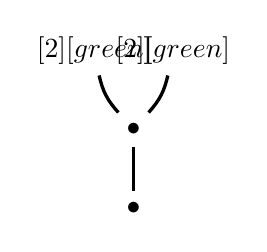
\begin{tikzpicture}[very thick, scale=0.5]
\node (foot) at (2,0) {$\bullet$};
\node (N1) at (2,2) {$\bullet$};
\node (N2) at (3,4) {$\Smiley[2][green]$};
\node (N3) at (1,4) {$\Smiley[2][green]$};
\draw (foot) -- (N1);
\draw (N1) to [bend right =15] (N2);
\draw (N1) to  [bend left=15](N3);
\end{tikzpicture}
\caption{\label{fig:HM}}
The state of the hydra after $M$ rounds.
% The hydra \texttt{h} of the proof that \(\omega^2\) is too small for proving Hercules' victory

\end{figure}


\begin{figure}[htb]
\centering
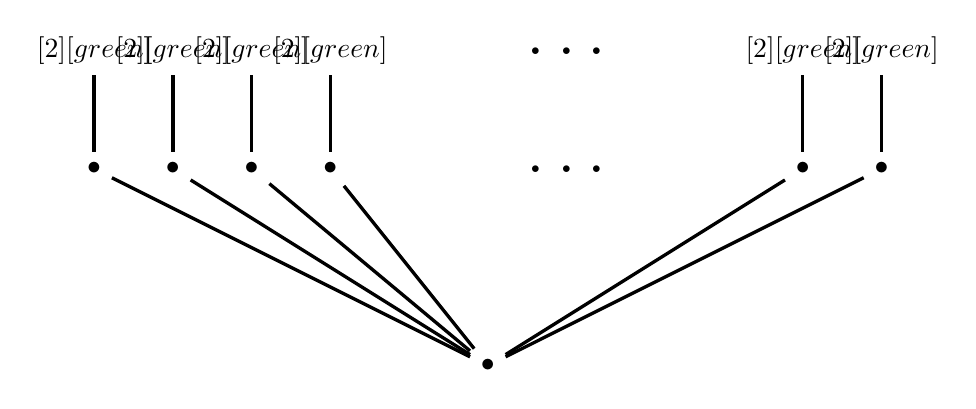
\begin{tikzpicture}[very thick, scale=0.5]
\node (foot) at (10,0) {$\bullet$};
\node (N1) at (0,5) {$\bullet$};
\node (N12) at (0,8) {$\Smiley[2][green]$};
\node (N2) at (2,5) {$\bullet$};
\node (N22) at (2,8) {$\Smiley[2][green]$};
\node (N3) at (4,5) {$\bullet$};
\node (N32) at (4,8) {$\Smiley[2][green]$};
\node (N4) at (6,5) {$\bullet$};
\node (N42) at (6,8) {$\Smiley[2][green]$};

\node (Ndots) at (12,8) {\Huge $\dots$};
\node (Ndots2) at (12,5) {\Huge $\dots$};

\node (N8) at (18,5) {$\bullet$};
\node (N82) at (18,8) {$\Smiley[2][green]$};
\node (N9) at (20,5) {$\bullet$};
\node (N92) at (20,8) {$\Smiley[2][green]$};


\draw (foot) -- (N1);
\draw (foot) -- (N2);
\draw (foot) -- (N3);
\draw (foot) -- (N4);
\draw (foot) -- (N8);
\draw (foot) -- (N9);
\draw (N1) to  (N12);
\draw (N2) to  (N22);
\draw (N3) to  (N32);
\draw (N4) to  (N42);
\draw (N8) to  (N82);
\draw (N9) to  (N92);
\end{tikzpicture}
\caption{\label{fig:HM-plus1}}
The state of the hydra after $M+1$ rounds (with $M+1$ heads). 

\end{figure}

\begin{Coqsrc}
Lemma L2_95_S : reachable (S M) 0 (S M) 0.
Proof.
  eright.
  - apply L2_95.
  -  left; constructor 3.
Qed.
\end{Coqsrc}


Then, applying once more the lemma \texttt{BigStep}, we get the exact time when
Hercules wins!


\begin{Coqsrc}
Definition N :=   iterate doubleS (S M) (S M).

Theorem   SuperbigStep : reachable N  0 0 0 .
Proof.
  apply Bigstep, L2_95_S.
Qed.
\end{Coqsrc}

We are now able to prove formally that the considered battle is 
composed of $N$ steps.

\begin{Coqsrc}
Lemma Almost_done :
  battle standard 3 (hyd 3 0 0) N (hyd 0 0 0).
Proof. 
  apply steps_battle, SuperbigStep.
Qed.

Theorem  Done :
  battle standard 0 hinit N head.
Proof.
  eapply battle_trans.
  -   apply Almost_done.
  -  apply L_0_3.
Qed.
\end{Coqsrc}



\subsection{A minoration lemma}

Now, we would like to get an intuition of  how big the number $N$ is.
For that purpose, we use a minoration of the function \texttt{doubleS} by the
function (\texttt{fun n => 2 * n}).

\begin{Coqsrc}
Definition exp2 n := iterate (fun n => 2 * n) n 1.
\end{Coqsrc}
Using some facts (proven in \url{../src/html/BigBattle.html}),we get several  minorations.

\begin{Coqsrc}
Lemma minoration_0 : forall n,  2 * n <= doubleS n.

Lemma minoration_1 : forall n x, exp2 n * x <= iterate doubleS n x.

Lemma minoration_2 : exp2 95 * 95 <= M.

Lemma minoration_3 : exp2 (S M) * S M <= N.

Lemma minoration : exp2 (exp2 95 * 95) <= N.
\end{Coqsrc}


The number $N$ is greater than or  equal to $2^{2^{95}\times 95}.$ If we wrote $N$ in base $10$, $N$ would require at least $10^{30}$ digits!


\section{Generic properties}


The example we just studied shows that the termination of any battle may take a very long time. If we want to study hydra battles in general, we have to consider 
any hydra and any strategy, both for Hercules and the hydra itself. So, we first  give some definitions, generally borrowed from transition systems vocabulary (see~\cite{tel_2000} for instance).


\subsection{Liveliness}


Let $B$ be an instance of \texttt{Battle}. We say that $B$ is \emph{alive} if
for any configuration $(i,h)$, where $h$ is not a head, there exists a further step in class $B$.


\vspace{4pt}
\emph{From Module~\href{../src/html/hydras.Hydra.Hydra_Definitions.html\#Alive}{Hydra.Hydra\_Definitions}}

\begin{Coqsrc}
Definition Alive (B : Battle) :=
  forall i h, 
     h <> head -> {h' : Hydra |  B i h h'}.
\end{Coqsrc}

The theorems \texttt{Alive\_free} and \texttt{Alive\_standard} of the module 
\url{../src/html/hydras.Hydra.Hydra_Theorems.html} show that the classes \texttt{free} and \texttt{standard} satisfy this property.

\begin{Coqsrc}
Theorem Alive_free: Alive free.

Theorem Alive_standard: Alive standard.  
\end{Coqsrc}

Both theorems are proved with the help of the  following strongly specified function:

\vspace{4pt}
\emph{From Module~\href{../src/html/hydras.Hydra.Hydra_Lemmas.html\#next_round_dec}{Hydra.Hydra\_Lemmas}}

\begin{Coqsrc}
Definition  next_round_dec n :
 forall h , (h = head) + {h' : Hydra & {R1 h h'} + {R2  n h  h'}}.
\end{Coqsrc}


\subsection{Termination}

The termination of all battles is naturally expressed by the predicate \texttt{well\_founded} defined in the module \href{https://coq.inria.fr/distrib/current/stdlib/Coq.Init.Wf.html}{Coq.Init.Wf} 
 of the Standard Library.

\index{Predicates!Termination}

\begin{Coqsrc}
Definition Termination :=  well_founded (transp _ round).
\end{Coqsrc}


Let $B$ be an instance of class \texttt{Battle}. A \emph{variant} for $B$ consists
in a well-founded relation $<$  on some type \texttt{A}, and a function
(also called a \emph{measure}) \texttt{m:Hydra->A} such that for any successive steps $(i,h)$ and $(1+i,h')$  of a battle in $B$, the inequality $m(h')<m(h)$ holds.


\vspace{4pt}
\emph{From Module~\href{../src/html/hydras.Hydra.Hydra_Definitions.html\#Hvariant}{Hydra.Hydra\_Definitions}}
\index{Coq!Techniques!Type classes}
\label{sect:hvariant-def}

\begin{Coqsrc}
Class Hvariant {A:Type}{Lt:relation A}(Wf: well_founded Lt)(B : Battle)
  (m: Hydra -> A):   Prop :=
  {variant_decr :forall i h h',
      h <> head ->
      battle_r  B i  h h' -> Lt (m h') (m h)}.
\end{Coqsrc}  

\index{Exercises}

\begin{exercise}
 Prove that, if there is an instance of (\texttt{Hvariant Lt wf\_Lt $B$ $m$}), then there exists no infinite battle in  $B$.
\end{exercise}




\subsection{Two small proofs of impossibility}
\index{Maths!Proofs of impossibility}

When one wants to prove a termination theorem with the help of a variant, 
one has to consider first a well-founded set $(A,<)$, then a strictly decreasing measure on this set.  The following two lemmas show that if  the order structure $(A,<)$ is too simple, it is useless to look for a convenient measure, which simply no exists. Such kind of result is useful, because it saves you time and effort.

\subsubsection{No variant on Peano.lt}
\label{omega-case}

The best known well-founded order is the natural order on the set $\mathbb{N}$ of natural numbers (the type \texttt{nat} of Standard library). It would be interesting to look for some measure $m:\texttt{nat}\arrow\texttt{nat}$ and prove it is a variant.

Unfortunately, we can prove that 
\emph{no} instance of class \texttt{WfVariant round Peano.lt $m$} can be built, where
$m$ is \emph{any} function of type \texttt{Hydra $\arrow$ nat}.



Let us present the main steps of that proof, the script of which  is in the module ~\href{../src/html/hydras.Hydra.Omega_Small.html}{Hydra/Omega\_Small.v} \footnote{ The name of this file means ``the ordinal $\omega$ is too small for proving the termination of [free] hydra battles ''. In effect, the elements of $\omega$, considered as a set, are just the natural numbers (see next chapter for more details)}.

%\subsubsection{Preliminaries}


Let us assume there is a variant $m$ from \texttt{Hydra} into \texttt{nat} for proving
    the  termination of all hydra battles.

\begin{Coqsrc}
Section Impossibility_Proof.
 Variable m : Hydra -> nat.
 Hypothesis Hvar : Hvariant lt_wf free m.
\end{Coqsrc}

We define an injection from the type \texttt{nat} into \texttt{Hydra}.
For any natural number $i$, $\iota(i)$ is the hydra composed of a foot and
$i+1$ heads at height $1$. For instance, Fig.~\ref{fig:flower} represents the hydra $\iota(3)$.

\begin{figure}[htb]
\centering
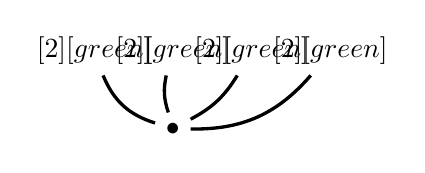
\begin{tikzpicture}[very thick, scale=0.5]
\node (foot) at (4,0) {$\bullet$};
\node (N1) at (2,2) {$\Smiley[2][green]$};
\node (N2) at (4,2) {$\Smiley[2][green]$};
\node (N3) at (6,2) {$\Smiley[2][green]$};
\node (N4) at (8,2) {$\Smiley[2][green]$};
\draw (foot) to [bend left =25] (N1);
\draw (foot) to [bend left =15] (N2);
\draw (foot) to [bend right =15] (N3);
\draw (foot) to [bend right =25] (N4);
\end{tikzpicture}
\caption{\label{fig:flower}
The hydra $\iota(3)$}
\end{figure}

  \begin{Coqsrc}
  Let iota (i: nat) := hyd_mult head (S i).    
  \end{Coqsrc}

Let us consider now some hydra \texttt{big\_h} out of the range of the injection $\iota$ (see Fig.~\vref{fig:h-omega-omega}).

\begin{figure}[htb]
\centering
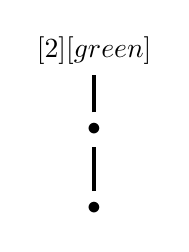
\begin{tikzpicture}[very thick, scale=0.5]
\node (foot) at (2,0) {$\bullet$};
\node (N1) at (2,2) {$\bullet$};
\node (N2) at (2,4) {$\Smiley[2][green]$};
\draw (foot) -- (N1);
\draw (N1) to  (N2);
\end{tikzpicture}
\caption{\label{fig:h-omega-omega}}
 The hydra \texttt{big\_h}.
\end{figure}

 \begin{Coqsrc}
  Let big_h := hyd1 (hyd1 head).
 \end{Coqsrc}

 Using the functions $m$ and $\iota$, we define a second hydra \texttt{small\_h}, and show
 there is a one-round battle that transforms \texttt{big\_h} into \texttt{small\_h}. Please note that,
due to the hypothesis \texttt{Hvar}, we are interested in the termination of \emph{free} battles. 
There is no problem to consider a round with \texttt{m big\_h} as replication factor.

  \begin{Coqsrc}
 Let small_h := iota (m big_h).
   
 Fact big_to_small : big_h -1-> small_h.
 Proof.
      exists (m big_h); right; repeat constructor.     
 Qed.
    \end{Coqsrc}
 
But, by hypothesis, $m$ is a variant. Hence, we infer the following inequality.


 \begin{Coqsrc}
Lemma m_lt : m small_h < m big_h.
 \end{Coqsrc}

In order to get a contradiction, it suffices to  prove the inequality
\texttt{m big\_h <= m small\_h}, i.e.,  \texttt{m big\_h <= m (iota (m big\_h))}.

More generally, we prove the following lemma: 

\begin{Coqsrc}
Lemma m_ge : forall i:nat , i <= m (iota i).
\end{Coqsrc}

Intuitively, it means that, from any hydra of the form (\texttt{iota $i$}), the battle will 
take (at least) $i$ rounds. Thus the associated measure cannot be less than $i$.
Technically, we prove this lemma by Peano induction on $i$.

\begin{itemize}
\item The base case $i=0$ is trivial
\item Otherwise, let $i$ be any natural number and assume  the inequality
  $i \leq m(\iota(i))$.
  \begin{enumerate}
  \item  But the hydra $\iota(S(i))$ can be transformed in one round into
    $\iota(i)$ (by losing its righmost head, for instance)
  \item Since $m$ is a variant, we have $m(\iota(i)) < m(\iota(S(i)))$,
    hence  $i< m(\iota(S(i)))$, which implies  $S(i)\leq  m(\iota(S(i)))$.
  \end{enumerate}
\end{itemize}

 Then our proof is almost finished.
 
   \begin{Coqsrc}
Theorem Contradiction : False.
Proof.
 apply (Nat.lt_irrefl (m big_h));
   apply  Lt.le_lt_trans with (m small_h).
  - apply m_ge.
  - apply m_lt.
Qed. 

End Impossibility_Proof.
\end{Coqsrc}

\index{Exercises}

\begin{exercise}
Prove that there exists no variant $m$ from \texttt{Hydra} into \texttt{nat} for proving
    the  termination of all \emph{standard} battles.
\end{exercise}





\subsubsection{Lexicographic order on \texorpdfstring{nat*nat}{nat*nat}}
\label{omega2-case}

We  prove now that even the type \texttt{nat * nat}, provided with the lexicographic product of \texttt{(nat,<)} by itself is too simple for proving the termination of all hydra battles. This impossibility result will prevent us from considering measures like the following one:


  \begin{Coqsrc}
  Let m h = (height h, hsize h).
  \end{Coqsrc}

The proof we are going to develop has exactly the same structure as in Section~\ref{sect:omega:case}


previous one. Nevertheless, the proof of technical  lemmas is a little more complex, due to 
 the structure of the lexicographic order on $\mathbb{N}\times\mathbb{N}$. 
Consider for instance that there exists an infinite number of pairs between
$(1,0)$ and $(2,0)$.


\begin{remark}
  The order structure we consider in this section is also known as the ordinal
  $\omega^2$. We identify any pair $(i,j)\in \mathbb{N}\times\mathbb{N}$ with the ordinal $\omega\times i + j$. Thus the three kinds of ordinals in $\omega^2$
  are represented as follows:
  \begin{description}
  \item[null ordinal] : the pair $(0,0)$
  \item[successor ordinal] : any pair $(i,j)$ where $j>0$
  \item[limit ordinal] : any pair $(i,0)$ where $i>0$
  \end{description}
\end{remark}

The detailed  proof script is in the file \url{../src/html/hydras.Hydra.Omega2_Small.html}.

\subsubsection{Preliminaries}
Let us assume there is a variant from \texttt{Hydra} into \texttt{nat*nat} (with the
   lexicographic ordering)  for proving the   termination of all hydra battles.

\vspace{4pt}
\emph{From Module~\href{../src/html/hydras.Hydra.Omega2_Small.html}{Hydra.Omega2\_Small}}


\begin{Coqsrc}
  Section Impossibility_Proof.
  
  Let t := (nat * nat)%type. 

  (** non-dependent lexicographic strict ordering on nat*nat *)
  
  Let lt2 : relation t := lexico Peano.lt Peano.lt.

  Infix "<" := lt2.
  
  (** reflexive closure of lt2 *)
  Let le2 := clos_refl _ lt2.
  Infix "<=" := le2.

  Variable m : Hydra -> t.
  
  Context (Hvar : Hvariant lt2_wf free m).
\end{Coqsrc}


Let us follow the same pattern as in Sect.~\ref{omega-case}.
First, we define an injection from type \texttt{t} into \texttt{Hydra}, by
 associating to  any pair $(i,j)$ the hydra with $i$ branches of length $2$ and
$j$ branches of length $1$.

%% revenir ici

\vspace{4pt}
\emph{From Module ~\href{../src/html/hydras.Hydra.Omega2_Small.html\#iota}{Hydra.Omega2\_Small}}

\begin{Coqsrc}
  Let iota (p: t) := 
    node (hcons_mult (hyd1 head) (fst p)
                     (hcons_mult head (snd p) hnil)).
\end{Coqsrc}

For instance, Figure~\vref{fig:essai2} shows the hydra associated to the pair
$(3,5)$. 

\begin{figure}[htb]
\centering
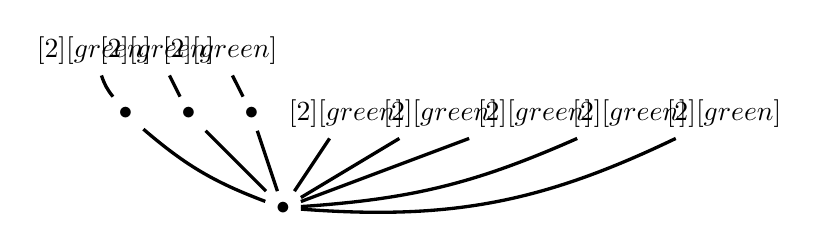
\begin{tikzpicture}[very thick, scale=0.4]
\node (foot) at (6,0) {$\bullet$};
\node (N1) at (1,3) {$\bullet$};
\node (N2) at (3,3) {$\bullet$};
\node (N3) at (5,3) {$\bullet$};
\node (N4) at (8,3) {$\Smiley[2][green]$};
\node (N5) at (11,3) {$\Smiley[2][green]$};
\node (N6) at (14,3) {$\Smiley[2][green]$};
\node (N7) at (17,3){$\Smiley[2][green]$};
\node (N8) at (20,3){$\Smiley[2][green]$};
\node  (N9) at (0,5) {$\Smiley[2][green]$};
\node (N10) at (2,5) {$\Smiley[2][green]$};
\node (N11) at (4,5) {$\Smiley[2][green]$};
\draw (foot) to [bend left=10] (N1);
\draw (foot) -- (N2);
\draw (foot) -- (N3);
\draw (foot) -- (N4);
\draw (foot) -- (N5);
\draw (foot) -- (N6);
\draw (foot) to [bend right=10] (N7);
\draw (foot) to [bend right=15] (N8);
\draw (N1) to [bend left=10] (N9);
\draw (N2) -- (N10);
\draw (N3) -- (N11);
\end{tikzpicture}
\caption{\label{fig:essai2}
The hydra $\iota(3,5)$}
\end{figure}




Like in Sect.~\ref{omega-case}, we build a hydra out of the range of \texttt{iota} (represented in Fig.~\vref{fig:h-omega2-small}).

\begin{figure}[htb]
\centering
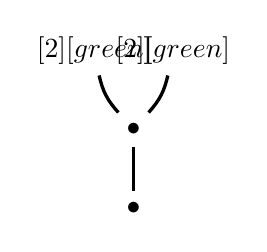
\begin{tikzpicture}[very thick, scale=0.5]
\node (foot) at (2,0) {$\bullet$};
\node (N1) at (2,2) {$\bullet$};
\node (N2) at (3,4) {$\Smiley[2][green]$};
\node (N3) at (1,4) {$\Smiley[2][green]$};
\draw (foot) -- (N1);
\draw (N1) to [bend right =15] (N2);
\draw (N1) to  [bend left=15](N3);
\end{tikzpicture}
\caption{\label{fig:h-omega2-small}}
 The hydra \texttt{big\_h}.
\end{figure}
\begin{Coqsrc}
   Let big_h := hyd1 (hyd2 head head).  
 \end{Coqsrc}
 
 In a second step, we build a ``smaller'' hydra.
 
\begin{Coqsrc}
   Let small_h := iota (m big_h).
\end{Coqsrc}

Like in Sect.~\ref{omega-case}, we prove the double inequality \texttt{m big\_h <= m small\_h < m big\_h}, which is impossible.

\subsubsection{Proof of the inequality \texttt{m small\_h < m big\_h}}

For proving the inequality  \texttt{m\_lt: m small\_h < m big\_h}, it suffices to
build a battle transforming \texttt{big\_h} into \texttt{small\_h}.

First we prove that \texttt{small\_h} is reachable from \texttt{big\_h} in one or two steps. Let us decompose \texttt{m big\_h}
into the pair $(i,j)$.
If $j=0$, then one round suffices to transform \texttt{big\_h} into $\iota(i,j)$.
If $j>0$, then a first round transforms \texttt{big\_h} into $\iota(i+1,0)$ and a second round into $\iota(i,j)$. So, we have the folowing result.

\begin{Coqsrc}
 Lemma big_to_small: big_h -+-> small_h.
\end{Coqsrc}

Since $m$ is a variant, we infer the following inequality:

\begin{Coqsrc}
Corollary m_lt : m small_h < m big_h.
\end{Coqsrc}


\subsubsection{Proof of the inequality \texttt{m big\_h <= m small\_h} }


The proof of the inequality \texttt{m big\_h <= m small\_h} is quite more complex than in Sect~\ref{omega-case}.  If we consider some pair $(i,j)$, where $i>0$, there exists an infinite number of
pairs stricly less than $(i,j)$, and there exists an infinite number of battles that start from
$\iota(i,j)$. In effect, at any configuration $\iota(k,0)$, the hydra can freely chose any replication number. Intuitively, the measure of such a hydra must be large enough for taking into account
all the possible battles issued from that hydra.
Let us give more technical details.

\begin{itemize}
\item The proof of the lemma \texttt{m\_ge : forall p : t,   p <= m (iota p)} uses well-founded induction on $p$, and not structural induction on natural numbers

\item For any pair $p$, we have to distinguish between three cases, according to the value of $p$'s components.
  \begin{itemize}
  \item $p=(0,0)$
  \item $p=(i,0)$, where $i>0$\,: $p$ corresponds to a limit ordinal
  \item $p=(i,j)$, where $j>0$\,: $p$ is the successor of $(i,j-1)$.
  \end{itemize}
\end{itemize}

Before starting the proof, we have to express the notion of \emph{limit} in terms of
least upper bounds, through the following logical equivalence.

\vspace{4pt}
\emph{From Module ~\href{../src/html/hydras.Hydra.Omega2_Small.html\#limit_is_lub}{Hydra.Omega2\_Small.v}}.

\begin{Coqsrc}
Lemma limit_is_lub : forall i p, 
   (forall j, (i,j) < p) <-> (S i, 0) <= p.  
\end{Coqsrc}

Let us define the notion of elementary ``step'' of decreasing sequences in
\texttt{t}


\begin{Coqsrc}
Inductive step : t -> t -> Prop :=
| succ_step : forall i j,  step (i, S j) (i, j)
| limit_step : forall i j, step (S i, 0) (i, j).
\end{Coqsrc}

The following lemma establishes a correspondance between the relation
\texttt{step} and hydra battles.

\begin{Coqsrc}
Lemma step_to_battle : forall p q, step p q -> iota p -+-> iota q.
\end{Coqsrc}

\index{Maths!Transfinite induction}

Thus, starting from any inequality $q < p$ on type \texttt{t}, we can build 
by transfinite induction over \texttt{p} a battle 
that transforms the hydra $\iota(p)$ into $\iota(q)$.

\vspace{4pt}
\emph{From Module~\href{../src/html/hydras.Hydra.Omega2_Small.html\#m_ge}{Hydra.Omega2\_Small}}

\begin{Coqsrc}
Lemma m_ge : forall p : t,   p <= m (iota p).
Proof.
  intro p ; pattern p;
    apply  well_founded_induction with 
               (R := lt2) (1:= wf_lexico lt_wf lt_wf);
     intros (i,j) IHij (* rest of proof skipped *)
\end{Coqsrc}

\begin{Coqanswer}
  i, j : nat
  IHij : forall y : t, y < (i, j) -> y <= m (iota y)
  ============================
  (i, j) <= m (iota (i, j)) 
\end{Coqanswer}


Then we have  three cases to consider, according to the values of $i$ and $j$.
\begin{itemize}
\item If $p=(0,0)$ then obviously, $\iota(p)\geq p = (0,0)$
\item If  $p=(i+1,0)$ for some $i\in\mathbb{N}$, we
 remark  that $p$ is strictly greater than any pair $ (i, j)$, where $j$ 
is any natural number.

Applying the battle rules, for any $j$, we have $\iota(i+1,j)  {\round} \iota(i, j) $, thus $m(\iota(p)) > m(\iota(i,j)$ since  $m$ is assumed to be a variant.

Applying the induction hypothesis, we get the inequality
 $ m(\iota(i,j)) \geq (i,j)$ for any $j$. 

Thus, $m(\iota(p)) > (i,j)$ for any $j$.
Applying the lemma \texttt{limit\_is\_lub}, we get  the inequality
$\iota(i+1,0)\geq (i+1,0)$

\item If $p=(i,j+1)$ with $j\in\mathbb{N}$, we have  $\iota(p)  {\round} \iota(i, j) $,
hence $m(\iota(p))> m(\iota(i,j)) \geq (i,j)$, thus $m(\iota(p))\geq (i,j+1)=p$

\end{itemize}

\subsubsection{End of the proof}

Since $<$ is a strict order (irreflexive  and transitive) on \texttt{nat*nat}, we can conclude that there is no
variant for termination on the lexicographic square of $(\mathbb{N},<)$.

\begin{enumerate}
\item From \texttt{m\_lt}, we infer the strict inequality 
\texttt{m small\_h < m big\_h}
\item from \texttt{m\_ge}, we get \texttt{m big\_h <= m (iota (m big\_h)) = m small\_h} 
\end{enumerate}


\vspace{4pt}
\emph{From Module~\href{../src/html/hydras.Hydra.Omega2_Small.html}{Hydra.Omega2\_Small}}

\begin{Coqsrc}
Theorem Impossible : False.
Proof.
  destruct (StrictOrder_Irreflexive  (m big_h)).
  apply le2_lt2_trans with (m small_h).
  -  unfold small_h;  apply m_ge.
  -  apply m_lt. 
Qed. 

End Impossibility_Proof.
\end{Coqsrc}

\index{Exercises}

\begin{exercise}
Prove that there exists no variant $m$ from \texttt{Hydra} into \texttt{nat*nat} for proving
    the  termination of all \emph{standard} battles.
\end{exercise}



\begin{remark}
In Chapter~\ref{ks-chapter}, we will prove a much more general  theorem
than the two previous results about $\mathbb{N}$ and $\mathbb{N}\times\mathbb{N}$. The proof of that general  result will share the same structure, but will 
require a lot of technical results. 
\end{remark}

\index{Exercises}
\begin{exercise}

\label{sec:orgheadline63}
Write \emph{direct} proofs ({i.e.},  without applying the result and tools of Chap.~\ref{ks-chapter}) that the following data structures  are too simple for defining a variant for any hydra battle.

\begin{itemize}
\item  $\omega^n$ : the set of all $n$-uples of natural numbers, ordered  by 
  lexicographic ordering
\item  $\omega^\omega$: the set of all decreasing sequences (with respect to $\le$)  of natural numbers, ordered by lexicographic ordering on lists.

For instance, the following inequality holds:
\[\langle 4,3,3,3,3,3,3,2,2,2 \rangle\,<\,\langle 4,4,2 \rangle\]
\end{itemize}

  
\end{exercise}


\subsubsection{Conclusion}

In order to build a variant for proving the termination of all hydra battles, we need to consider order structures more complex than the usual order on type \texttt{nat}. 
The notion of \emph{ordinal number} provides a catalogue of well-founded order types.
For a reasonably large bunch of ordinal numbers, \emph{ordinal notations} are data-types which allow the \coq{} user to define functions, to compute and prove some properties, for instance by reflection.

So, the next chapters will present ordinal numbers and ordinal notations, and we will
look for a variant complex enough for proving the termination of all battles, but not too complex if possible.


